\documentclass[12pt]{article}
\usepackage[utf8]{inputenc}
\renewcommand{\familydefault}{\sfdefault}
\pagenumbering{gobble}
\usepackage{fullpage}
\usepackage{graphicx}
\usepackage{geometry}
\geometry{
  a4paper,
  top=1.2mm,
  bottom=1mm,
  }
\title{\huge{\textbf{CURRICULUM VITAE}}\vspace{-2.5ex}}
\date{}
\begin{document}
\maketitle
\section*{Datos personales}
\bgroup
\def\arraystretch{1.25}
\begin{tabular}{p{5cm} l}
  Nombres y apellido&Martín Roberto Rossi\\
  Fecha de nacimiento&28 de enero de 1991\\
  Edad&30 años\\
  Lugar de nacimiento&Venado Tuerto\\
  D.N.I. número&36.038.116\\
  Estado civil&Soltero\\
  Teléfono&3462-542608 / 427383\\
  Correo electrónico&martinros24@gmail.com\\
\end{tabular}
\setlength{\unitlength}{0.5cm}
%% \begin{picture}(5,5)
%% \put(3.5,-3.5){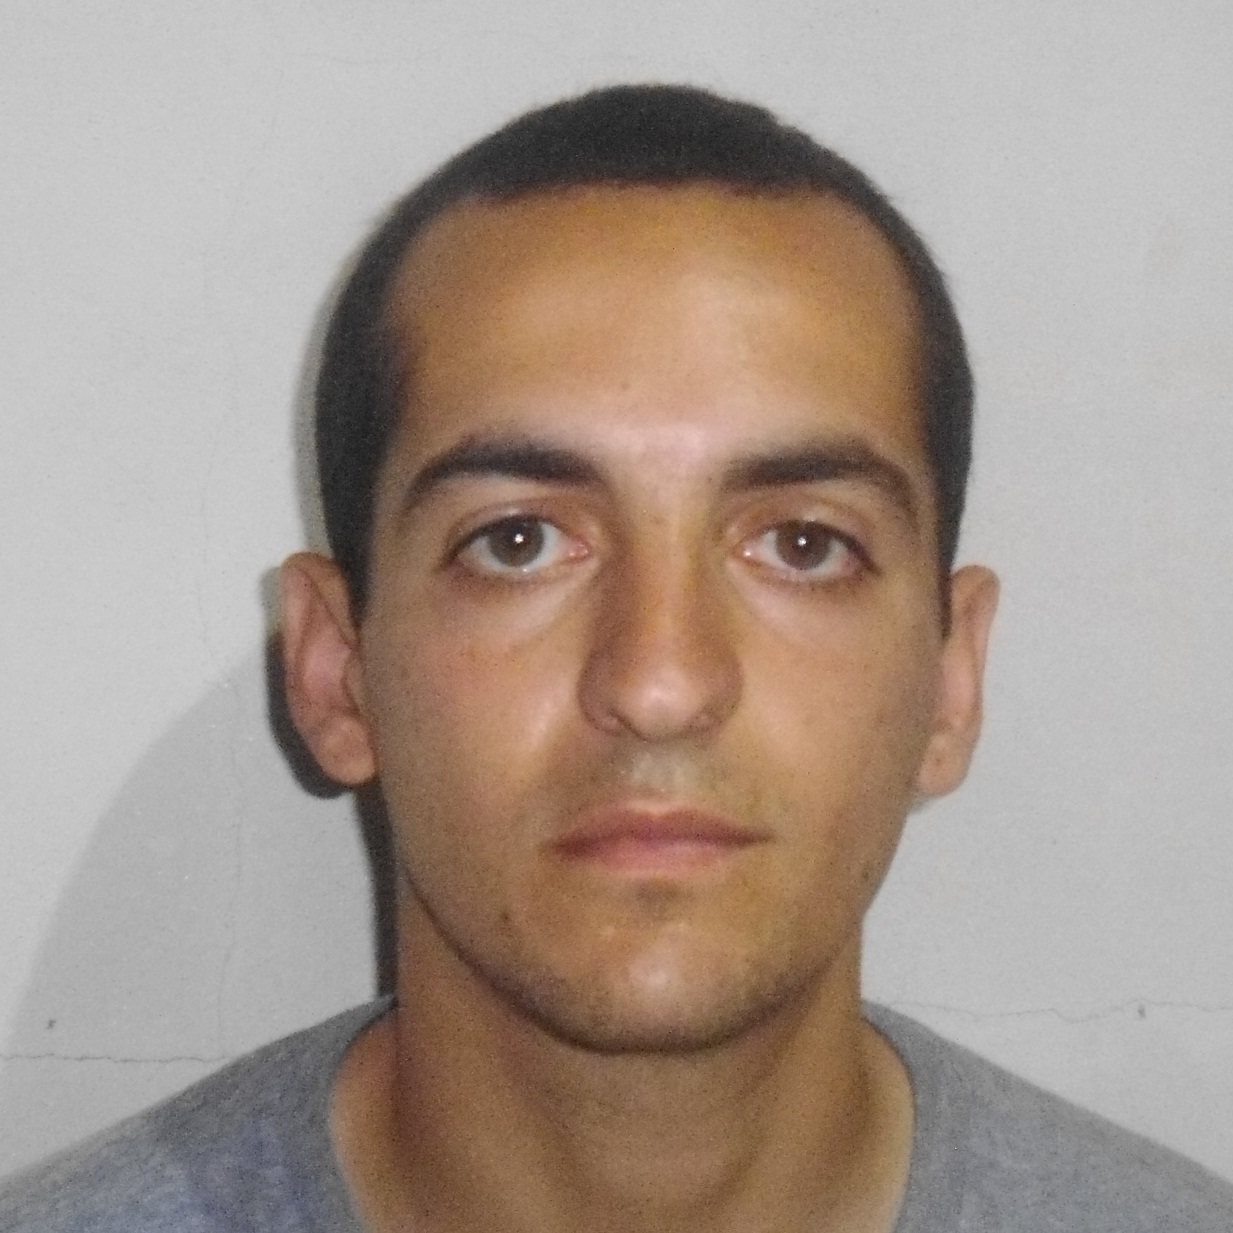
\includegraphics[width=4cm,clip=true]{face_c}}
%% \end{picture}
\subsection*{Formación académica}
\begin{tabular}{p{3.8cm} l}
  \multicolumn{2}{l}{\textbf{Secundario}}\\
  2006-2008&Polimodal: modalidad economía y gestión.\\
           &\small{Colegio Sagrado Corazón, Venado Tuerto.}\\
  \multicolumn{2}{l}{\textbf{Terciario}}\\
  2009-2011, 2015-2016&Analista en computación administrativa.\\
           &\small{Instituto católico de enseñanza superior (ICES), Venado Tuerto.}\\
  \multicolumn{2}{l}{\textbf{Otros estudios}}\\
  2015&Curso: Experto universitario de seguridad de la información.\\
           &\small{Universidad Tecnológica Nacional (UTN).}\\
  2018&Diplomatura en programación Java.\\
           &\small{Universidad Tecnológica Nacional (UTN).}\\
  \multicolumn{2}{l}{\textbf{Estudios en curso}}\\
           &Licenciatura en ciencias de la computación.\\
           &\small{Facultad de ciencias exactas, ingeniería y agrimensura (FCEIA), Rosario.}\\
           &\small{Estado: Cursando tercer año.}\\
\end{tabular}
\subsection*{Idiomas}
\begin{tabular}{l l}
  Inglés&Nivel intermedio\\
\end{tabular}
\subsection*{Experiencia laboral}
\begin{tabular}{l l}
  2014-2021&Cadetería Serpet\\
\end{tabular}
\subsection*{Otros datos de interés}
\begin{tabular}{l}
  Carné de conducir B-1\\
\end{tabular}
\end{document}
